\documentclass{article}
\usepackage[utf8]{inputenc}

\title{MultiAgent Systems course project}
\author{Federico Vaccaro - Università degli Studi di Firenze }
\date{September 2020}

\usepackage{natbib}
\usepackage{graphicx}
\usepackage{amsmath}
\usepackage{algorithm}
\usepackage{float}
\usepackage{algpseudocode}
\begin{document}

\maketitle

\begin{abstract}
	The purpose of this project is to apply a reinforcement learning technique - the Deep Q-Learning - for allow an agent to learn how to reach a given arrival point in a grid-shaped space, while trying to take the minimum count of steps and avoiding obstacles.
\end{abstract}


\section{Introduction}

The three main paradigms of the Machine Learning are: \textbf{Unsupervised} learning, where the model try to understand the underlying distribution of the dataset without any other input aside from the data themselves; \textbf{Supervised} learning, where paired with each sample there is a label, and the learning algorithm tries to fit the distribution that bound each sample to its label; lastly, there is the \textbf{Reinforcement} learning, where given an \textit{agent} operating within an environment $\mathcal{E}
$, has to 'find' the \textit{best policy}, i.e. the agent should determine a sequence of steps for maximizing a \textit{cumulative sum of rewards} (and/or minimizing a punishment!) obtained at each time-step. The first difference that we observe, is the ambiguous definition of the problem: there is no explicit dataset and no labels, which makes at first glance unclear how formulating a \textbf{loss function} for driving the training. In fact, there are various strategy for tackling the problem: the most known are \textbf{value iteration}, \textbf{policy iteration} and \textbf{Q-Learning}. In this project, we focused on the application of the Q-Learning, however the three listed strategy have in common the property of respecting the \textbf{Bellman equation of Dynamic Programmming}. In this report, we will first formulate the DQL algorithm, then applying it to a game we designed.

\section{Problem formulation}

We consider tasks in which an agent interacts with an environment $\mathcal{E}$, in this case out \textit{GridWorld} game,
in a sequence of actions, observations and rewards. At each time-step the agent selects an action $a_{t}$ from the set of legal game actions, $A = \{1, . . . , K\}$. The action is passed to the emulator and
modifies its internal state and the game score. In general $\mathcal{E}$ may be stochastic. The emulator’s
internal state is not observed by the agent; instead it observes an image $s_t \in \mathbf{R}^d $ from the emulator. % which is a vector of raw pixel values representing the current screen.% 
In addition it receives a reward $r_t$ representing the change in game score. Note that in general the game score may depend on the
whole prior sequence of actions and observations; feedback about an action may only be received
after many time-steps have elapsed: \textit{e.g.} we will see that we designed our game to return a negatie reward if a cell has been already visited.  % nel nostro caso, se l'agente dopo un lungo giro torna al punto iniziale, la penalità sarà determinata dal fatto che l'agente ha visitato una cella molte azioni prima %

As previously stated, goal of the agent is to interact with the emulator by selecting actions in a way that maximises
future rewards. We make the standard assumption that future rewards are discounted by a factor of $\gamma$ per time-step, and define the future discounted return at time $t$ as $R_t = \sum_{t'=t}^{T}\gamma^{t'-t}r^{t'}$, where $T$
is the time-step at which the game terminates. With the discount factor, we discourage the agent to complete the task in too much steps (at $t'=+\infty$, there is no reward). We define the optimal action-value function $Q^\star(s, a)$ as the maximum expected return achievable by following any strategy, after seeing some state $s$ and then taking some action $a$, $Q^\star (s, a) = max_\pi \mathbf{E}[R_t |s_t = s, a_ t = a, \pi]$, where $\pi$ is a policy mapping sequences to actions (or distributions over actions).

The optimal action-value function obeys an important identity known as the (previsionale mentioned) \textbf{Bellman equation} (\ref{bellman-eq}). This is based on the following intuition: if the optimal value $Q^\star (s_0 , a_0 )$ of the sequence $s_0$ at the next
time-step was known for all possible actions $a_0$ , then the optimal strategy is to select the action $a_0$, maximising the expected value of $r + \gamma Q^\star (s_0, a_0)$
\begin{equation}
\label{bellman-eq}
	Q^\star (s,a) = \mathbf{E}_{s' \sim \mathcal{E}} [ r + \gamma \max_{a'} Q^\star(s', a') | s, a  ]
\end{equation}

\section{Deep Q-Learning}

We will use a function approximator (as neural networks, which we refer as \textit{Q-networks}), with parameters $\theta$, to approximate the action-value function.
\begin{equation}
	Q(s, a; \theta) \approx Q ^\star (s, a). 
\end{equation}
A Q-network can be trained by minimising a sequence of loss functions $L_i(\theta _i )$ that changes at each
iteration $i$.
\begin{equation}
\label{dql}
\begin{aligned}
	L_i(\theta _i ) = (y_i - Q(s,a|\theta_i))^2 \\
	y_i = \mathbf{E}_{s' \sim \mathcal{E}} [ r + \gamma \max_{a'} Q^\star(s', a'|\theta_{i-1}) | s, a  ]
\end{aligned}
\end{equation}
The formulation of the loss $L_i(\theta_i)$ in (\ref{dql}) is differentiable, thus we will apply a \textit{stochastic gradient descent} for minimizing 
Where the parameters $\theta_{i-1}$ are held fixed during the weights update; othewise, with a gradient descent step the target would also try to match the Q-network values, instead of the opposite. Note that this method is \textbf{model-free}, i.e. it has no prior knowledge/estimation of the emulator $\mathcal{E}$, but it directly observe its "external" state. Also, the method is \textbf{off-policy}, because it does not learn by directly sampling from a policy (a sequence of steps), but rather training on different actions, even randomly sampled.\\
Before introducing the final Deep Q-Learning algorithm, we first need to describe the \textbf{replay memory} and the \textbf{exploration-exploitation} technique for action sampling.
\subsection{Replay memory}
At each time-step, we collect a tuple from the experience of the agent: $e_t = (s_t, a_t, s_{t+1}, r_t)$. We mantain these experiences in a pool, which we refer as \textit{replay memory}, then as the training continues, we build a dataset of experiences. Then we are abilitated sample mini-batches of tuples from this dataset, making the reinforcement learning algorithm more similar to a "classic" supervised learning task. This is efficient for two reasons: first, it allows to build minibatches of \textbf{indipendent samples}, which are mandatory for a better estimation of the gradient via SGD; also it is \textbf{computationally-efficient}, since we can leverage parallel-computing hardware and optimized software.
\subsection{Exploration-exploitation}
During the training, we let the agent playing multiple matches, from where we collect experiences. However, especially in the first stages of the training, the agent does not know how the environment will change to a chosen action, nor the reward it will receive. Thus, it is reasonable to chose a random action instead of the action with maximum Q-score, in order to \textbf{explore} the states of the environment. Furthermore, in the very first stages the parameters are near from being random initialized, then the output Q-scores have really few sense. In order to achieving this, we select a probability $\epsilon$ with we select a random action ($1 - \epsilon$ selects the \textit{greedy} action) during the training. As the agent keep accumulating experience and training, $e$ will tend to decrease, letting the agent improving the learned policies. We refer to this mechanism as \textbf{exploration-exploitation}.\\
This strategy can also be interpreted from a \textbf{Global Optimization} perspective, as an "hill-climbing" method for exiting local minima, or similar to what is known in the Deep Learning community as parameters "warm-up".
\\
\\
Now, we are able to define the \textbf{Deep Q-Learning training algorithm}.
\subsection{Deep Q-Learning algorithm}
In the Alg. \ref{dqlalg} we show the pseudocode for the Deep-Q-Learning algorithm.
\begin{algorithm}[!h]
	\caption{Deep Q-Learning algorithm}
	\label{dqlalg}
	\begin{algorithmic}
		\State Initialize ReplayMemory $\mathcal{D}$ with capacity N
		\State Initialize DQN $Q(x, a|\theta)$ with random weights $\theta_0$
		\For{episode $1,M$}
		\State Initialize sequence $s_1=\{x_1\}$
		\For{$t=1,T$}
			\State With probability $\epsilon$ select action $a_t$ 
			\State otherwise select $a_t=\max_{a}Q(x_t, a|\theta)$
			\State Execute $a_t$ and observe reward $r_t$ and state change $x_{t+1}$
			\State set sequence $s_{t+1}=(x_t, a_t, x_{t+1}, r_t)$ 
			\State store sequence $s_{t+1}$ in $\mathcal{D}$
			\State sample a minibatch of transitions $s_j=(x_j, a_j, x_{j+1}, r_j)$
			\State set $y_j = 
			\begin{cases}
				r_t \text{ if $x_{t+1}$ is terminal} \\
				r_t + \gamma\max_{a'}Q(x_{t+1}, a'|\theta) \text{ otherwise}
			\end{cases}
			$
			\State Compute $L(\theta) = \sum_{j}^{B} \frac{1}{B} (y_j - Q(x_j, a_j|\theta) )^2 $
			\State Perform a gradient update based on $\nabla_\theta L\theta$
		\EndFor		
		\EndFor
	\end{algorithmic}
\end{algorithm}
% TODO

\section{Experimental results}
\subsection{GridWorld-style game}
For testing our implementation of the DQL algorithm, we implemented a game in a \textit{GridWorld} fashion. The game consists of a grid with shape $D \times D$, where we set $D = 16$. For enabling the rendering to an RGB image, each cell in the grid has $3$ channels (thus the state is a tensor $D \times D \times C$). By default, a cell is white (has value $1.0$ for each channel). Then, the agent should move its position, represented when a cell is \textit{green} colored to the red square which is the ending (winning) cell. Both start and ending positions are randomly generated at each match to be on the perimeter of the grid, but to be always distant)  Also, we generate a number of \textit{obstacles} uniformly spread across the grid, which are represented with the black color. The agent can move at each step the green square in one of the four direction (up, right, down, left).
The reward system works as follows:
\begin{itemize}
	\item $r_t = 1$ If the agent get the green closer to the ending square but in a white cell;
	\item $r_t = -1$ If the agent move the green square upon an obstacle;
	\item $r_t = -1$ If the agent enter again in an already visited cell (for discouraging loops) \textbf{or} try a move towards a wall ;
	\item $r_t = 2$ If the agent can reach the red square.
	\item $r_t = 0$ If the agent gets farther from the objective, but in a white cell. There is no penalty here for avoiding punishing the agent for going around an obstacle. We let the discount factor limiting the rewards for being obtained later.
\end{itemize}
This problem, can be interpreted as a different modeling of finding the \textbf{shortest-path} between two cells.

\subsection{Implementation details}
The network architecture we utilized is composed from one fully-connected (FC) hidden layer with 1024 output units, followed by a batch normalization layer which we found fundamental for regularization purposes, and a final FC layer for producing the Q-scores. After the hidden layer, is applied a ReLU function for obtaining non-linearity. The state tensor, which is the input of the network, is reshaped to a 1-d vector of dimension $768$. Summarizing, the computing pipeline is as in (\ref{net}). We did not find useful to include the last few frames (as is common practice) in the computing of the Q values, since the optimal solution does not depend on the previous steps.

\begin{equation}
\label{net}
	Q(\textbf{s}|\theta) = \textbf{s} \rightarrow FC_{1024} \rightarrow ReLU \rightarrow BN \rightarrow FC_{4}
\end{equation}
The network is trained for $500$ episodes. Each episode, the network is updated $1000$ times with the samples drawn from the Replay Memory in mini-batches of $32$. The discount factor is fixed $\gamma=0.9$ at The exploration rate $\epsilon$ starts at $0.9$, linearly decaying until the half-way episode to $0.1$. The employed optimization method is Adam, with \textit{learning rate} $\eta = 10^{-4}$ and \textit{weight decay} (L2 regularization) $= 10^{-6}$.
Before processing the state with the network, we normalize the state vector components in the range $[-1,1]$.
\begin{figure}[h!]
\centering
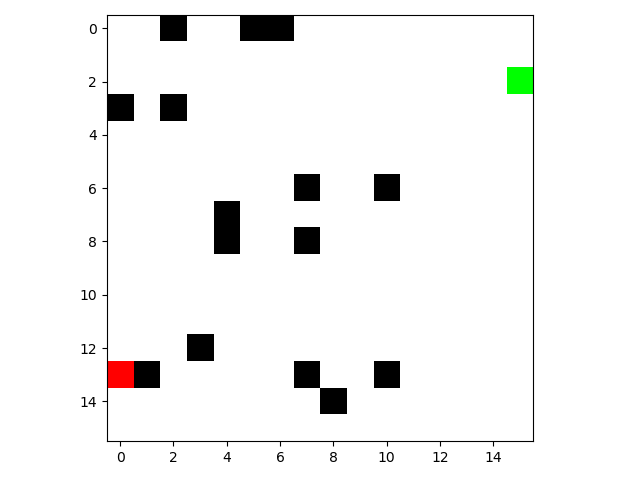
\includegraphics[width=\textwidth]{game_example}
\caption{Example of game initial state.}
\label{fig:game1}
\end{figure}

\section{Conclusion}
In this project, we experienced a different way of solving problem: the Reinforcement Learning, applying the Deep Q-Learning algorithm. In particular, we found interesting how a small neural network is able to successfully approximate a classic pathfinding algorithm \textit{e.g. Dijkstra, or the $A^\star$ algorithms} without explicitly coding its rules, but rather by designing a simple reward system. However, the real advantage of with this machine learning, is that we are potentially able approximate a wide range of tasks, not only the class of algorithms we saw in this experiment. 

\bibliographystyle{plain}
\bibliography{references}
\end{document}
